\chapter{Byers II Module}


\section{Lecture 5 - Differential geometry in ML}

\subsection{Introductory example}

When we think about mathematics, it has value in that we sort of can have very clearly defined true propositions. So we could say I can certainly write down some true propositions such as tautological things like 1=1, I could say obviously 2+2=4. And then I could say, oh, well, there's some obviously um counter examples. I could say it is false to say 1=100 or something, that doesn't make any sense. I can do 2+2=5, and we would all say, well, these are falsehoods. Right? Trivial. 

But actually let me ask you, are there any ways that I could make the things on the false side true? What makes—what could have I assumed over here that I'm not telling you about maybe over here, or I assumed different things over here that were different from what was assumed there to make these true statements? Anybody have any idea? Sure.




\begin{centering}
\begin{verbatim}
    True                         False

    1 = 1                       1 = 100
    2+2 = 4                     2 + 2 = 5
\end{verbatim}
\end{centering}
Think of it from a physics standpoint. As physicists, why can I make the stuff on the right true, whereas a mathematician will be upset regardless, usually.

'If they have large enough error bars, the result might be true.'

Yeah, that's right. You could have errors and uncertainties. And in fact, on this bottom one here, that's what I could say, like this number and this number are drawn from a Gaussian. Maybe it's centered at 2 and has some sigma that has some width to it. And now it is actually possible for me to draw two numbers from a Gaussian and add them together and there is a way for me to reach five or—or within some bound of five, right? So 2+2=5 within the framework of probability and uncertainty is completely possible. Okay? 

So what did it mean over here when I wrote 2+2=4 and thought it was a truth? What was I assuming about those numbers that we did not assume over there? Infinite precision? Right, we were assuming that the sigma here was implicitly going to zero. And so these numbers as real numbers were defined exactly. \textbf{In other words, these numbers had an infinite amount of information in them.} 

And if that sounds weird and possibly bad, you're right. Okay? Every number you have, you probably learned this in your undergraduate physics lab, you never report a single number, you always report two numbers. You say, well, here is essentially something like the mean and here is essentially something like the standard deviation of the variance. 

Now when you do mathematics and you represent numbers in the way mathematicians do, they tend not to think about that aspect of the number. But as physicists, natural scientists, people working with data in the world, we have to understand that uncertainty quantification is a very important part of our problem. And things that someone might say, well, that is a falsehood, aren't in the right context. Okay, so you got the slightly more complicated one right first. So how do I fix this one?

'Units.'

It's pretty silly, right? But it's not when you realize units matter. So when I use numbers in the world, I have to think about the units associated with them. Not just the uncertainties—that's important too—but the units. And imagine when I say I have to form a dimensionless constant and relate that to other dimensionless constants. In other words, I'm—I'm saying that for units that have dimensions and I have to combine them together in a way that perhaps the dimensions don't matter because they're arbitrary. You make up the dimensions. 

\textbf{So anything you can make up, the world doesn't really care about. It has to be invariant to those choices. So there are certain symmetries inside of the representations of numbers that we use in physics to represent the world that we have to account for and understand.} So one meter of course is 100 centimeters. It's trivial, you know, to write it like this. It looks like a trick, but it—it suggests an important change of your mindset to realize units, dimensionality, uncertainty quantification change what you think is true and false in a very strict mathematical sense. It opens your mindset up. And that's exactly what differential geometry does on a wider scale. Okay? 



\subsection{Differential geometry}
I promise this is not a philosophical lecture. But let—I want to get our conceptual positioning correct. Okay? And so, this is a famous line about language. The famous philosopher Wittgenstein at Cambridge many years ago said: 

\begin{centering}
\begin{verbatim}
'Philosophy is a battle against the bewitchment of our minds by language.' 
\end{verbatim}
\end{centering}
Okay? And this is just saying this like you start to think the words are real and you project reality onto the representation and you can get lost in the representation. 

Well, that is actually exactly what happened to physics prior to relativity. Physics became lost in the representations of the physics and didn't figure out how to abstract itself from those representations. And so, modifying what Wittgenstein said about um language, we can say that differential geometry is a battle against the bewitchment of our minds by coordinates. 

So these coordinate systems, right? And it's important that we need coordinate systems, they are not the enemy of what we are doing, they are a vital tool to have coordinate systems and use them. But it is vital that you not create properties that are inside your coordinate system because you get to make up your coordinate system, right? You choose the coordinate system. You choose to switch coordinate systems. 

Now what happens if the physics changed with your choice of coordinate system? This is a disaster. This means physics is not about the world, it's about stuff you choose in your head. And that's crazy. 

And this is what Einstein was really battling with when he was trying to create relativity. The challenge of relativity was that, and certainly special relativity stayed fairly trapped within its coordinate systems. Okay, you could think in terms of essentially Cartesian coordinates and do all of special relativity. But when Einstein attempted to generalize special relativity to general relativity and say, well, now we're going to include um forces and more rigorously and things like gravity, a very distinct problem emerged is that they—you're trapped inside choices of coordinate systems and struggling to figure out what is the coordinate system artifacts and what is the physics that lives beyond the coordinate system. Okay? 

You see the difference, right? There's many things you would calculate that you'd say: 'If I change coordinates, does this change too?' And does that change get reflected in the mathematics? So we have to be careful. Coordinate systems are very much like these choices of units or understanding whether the numbers we have have finite precision. \textbf{ Coordinate systems are also something that we assume and can build in artifacts and mistakes into our representations.} And I hope you start to see a hint of why this might matter in machine learning or data analysis.



\subsection{Recap: ML turns probabilistic problems into geometrical problems}

\begin{figure}[H]
    \centering
    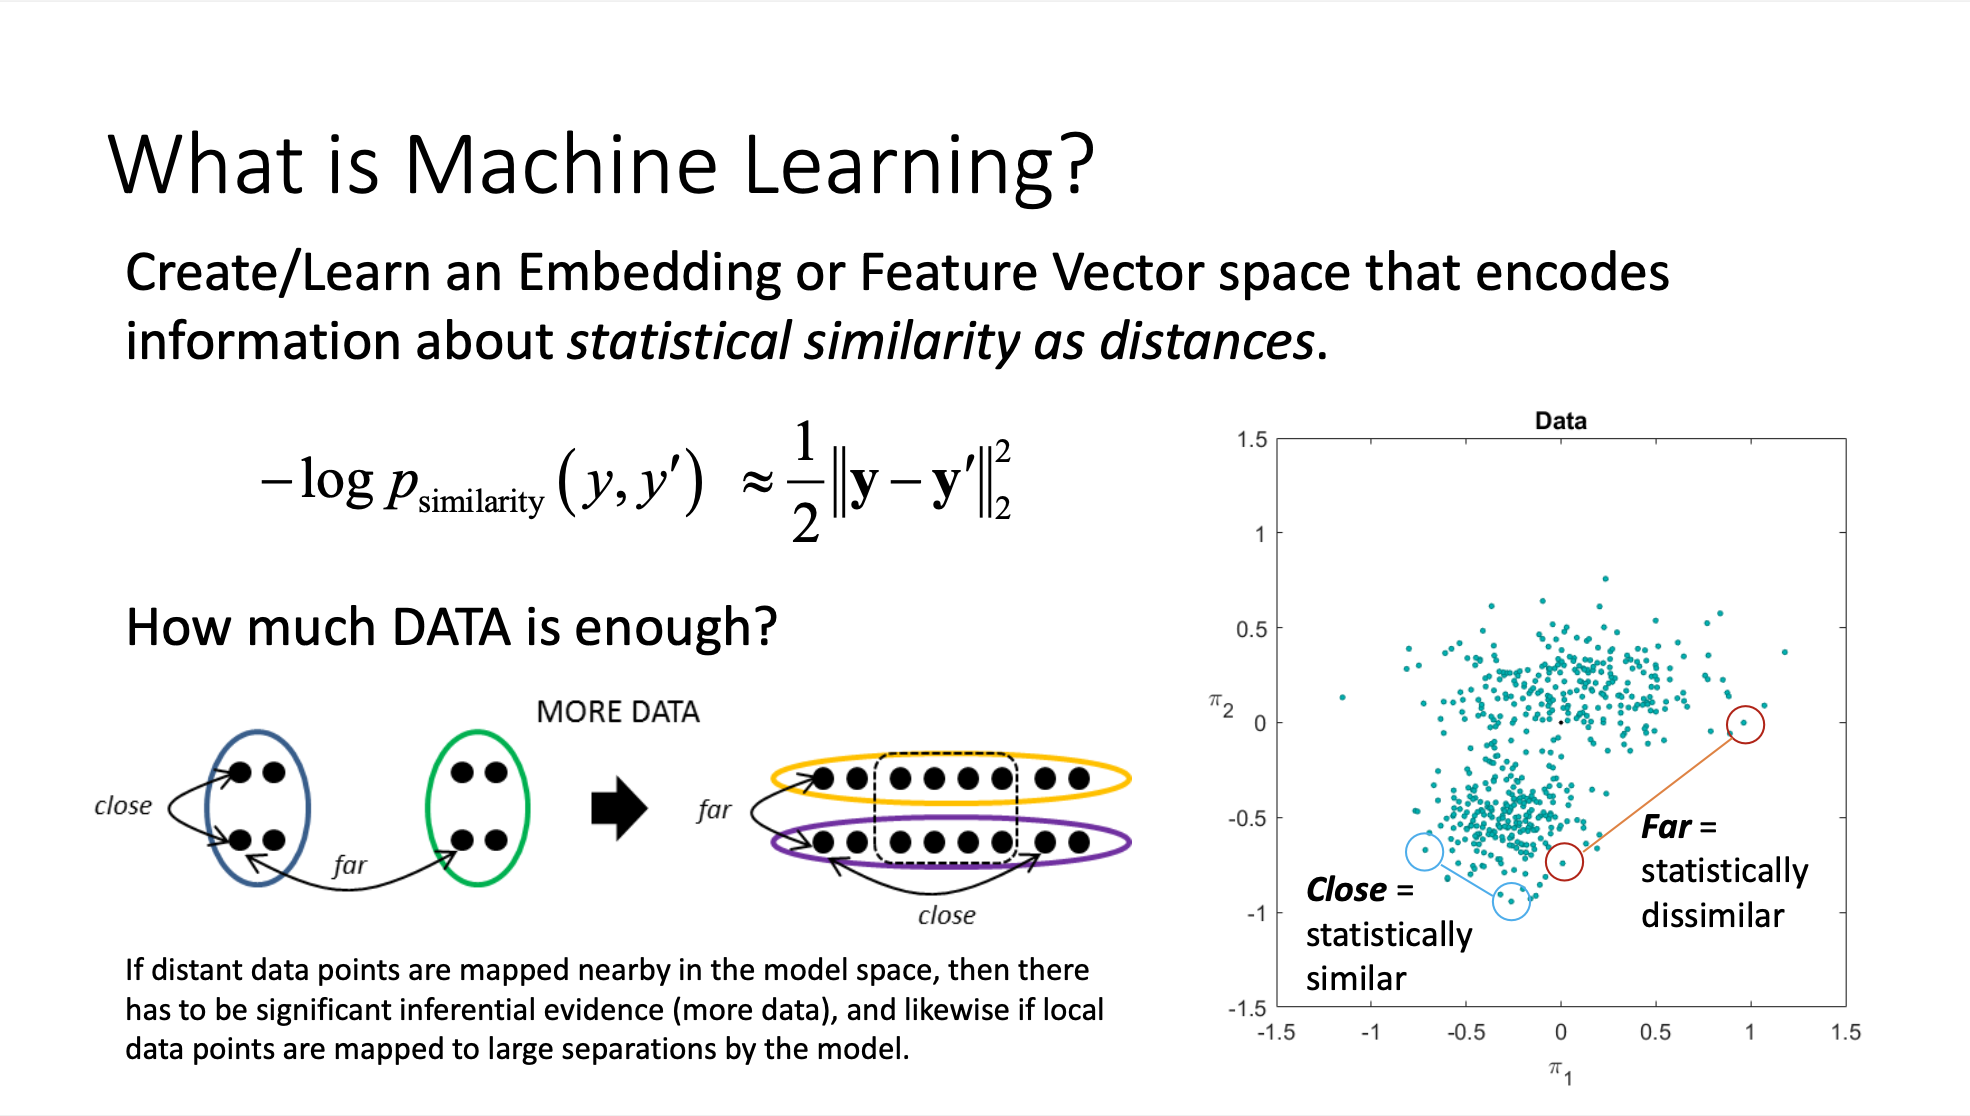
\includegraphics[width=\textwidth]{figures/B1_self_information_potential.png}
    \label{fig:self_information_potential}
    \caption{The self information potential $p_{similarity}(\mathbf{y}, \mathbf{y'})$ is the fundamental quantity}
\end{figure}

So let's remind ourselves. I—if you recall back,I was trying to say: 'Well, what is machine learning?'

So you've been exposed to information theory—a very peculiar science, a very confusing in its own right. It always seems to have the answers but never tells you them. It's like an oracle. And I'll come to why information theory is later in another lecture—why information theory is so problematic. And it has to do with the fact that in the world you never have the probability distributions, you have the data. And information theory works perfectly if you have the probability distributions, but it doesn't work so well if you just have the data. And I can show you how to try to fix that so that you can use information theory in a practical sense with data, which is something evidently they never want to talk about in information theory courses. But anyway. 

So this kind of information theoretic term, which is sometimes called, if you remember, the \textbf{self-information}. \textbf{I claimed in our discussion this is the smarter object to look at in many cases.} The probability itself is a little strange to think about. But this term, $-\log$, is actually more intuitive, especially for physicists, because this is essentially like a potential energy. \textbf{And it's the potential energy in which sits your data. And so this is the constraints that keeps your data organized in the space as if they were traveling particles doing Brownian motion traveling around in a potential.}
\medskip \newline
Now what does machine learning do? Machine learning says: 'Okay, I'm given this potential.' In fact, I would say any good physicist would probably do this too—Taylor expand it! Right? Let's expand this term and pick up the lead order term. Okay, the first non-trivial lead order term is this one where we say I've essentially expanded around some location and it's—it's like a harmonic oscillator, right? So from a physics standpoint, you should be like 'Sure.' This is a—a good starting point. The—it's like saying I have my potential that's holding my data together—let's imagine it's initially like a harmonic oscillator potential as the lead order non-trivial term of this expansion. 

And so this is an approximation and you say: 'Ah, great. I can take this probability of similarity.' This is where the interpretive part of the problem comes in. 

So what's happening is that the probability of similarity says that you give me an object, and you give me another object, and I have some measure of what I can see where I say: 'Are these objects similar or not with however I see them?' Okay. Um, if you remember in one of my earlier lectures, I called that \textbf{relevance}. What is the relevant thing I can see that's different? Because the brutal fact about all the data in the world is pretty much it's all different. 

Every—you could tell almost—I could tell every one of these tiles apart from each other, right? Every one of these is unique in some way and they could be uniquely identified. All the tiles in all the buildings in all the world. Now the question is: 'In what task would that be relevant? Would it matter that I could tell every tile apart?' Now there are tasks where it matters that I could tell your fingerprints apart, right? Or your facial features, right? 

So knowing that every one of you is different is important for some tasks. Other tasks I say: 'I detect a human, I detect a tile.' That is a sufficient level of classification. So it's relevant what task I do. 

\textbf{So when I say similarity here, I'm saying similarity with respect to doing something. A choice about what you do.} So you can almost always with very sophisticated visual systems like we have, you can always see difference. The question is: 'You have to see the difference and figure out which differences matter.' And that's what a classifier is. A classifier is figuring out the differences that matter that you can see. If you can't see them, it's obviously hopeless, you can't use those features. 

You want to say the distance—remember, machine learning is saying: 'I want to—probability's hard to work with. It's complicated computationally.' And what's—what's easy to work with? Remember, what is the—one of the fastest things we can do on computers? Numerical linear algebra. Okay? If you can convert a nasty probability problem into a numerical linear algebra problem, it's a big win—a very, very big win for you. And that's what machine learning exploits. It's one of its key differences with statistics, and why it came more from computer science. Computer scientists looked at large data sets and said: 'We will have to have computational efficiency,' and so how do you leverage things like numerical linear algebra? 

So now we took a problem that was over in a probability space with a probability rules, which are actually quite inconvenient often to work through (you know, they're only two rules, right? in terms of marginalization and completeness and things, but it actually creates a kind of calculus mess over there). And so here, we said: 'Now it's just distance.' And then what we did was—see the script Y and the—the bold-faced Y—is somehow—I mean, what—if I tell you I'm going to do distances between things, what does that mean? 

Well, it means they're \textbf{vectors}. They're like points in a space, like a vector space. And I say: 'Well, there's this rule, this Euclidean rule of take the coordinate'—and I'll say 'coordinate' with 'scare quotes' because of our differential geometry preamble—and we say: 'Okay, what is the distance between this point and this point just through the usual Euclidean way of subtracting the components-wise differences between each of those, and then we can add them up.' 

And so now we have a—a way of saying: 'Ah, I can create a space that this is in, my data, where I've mapped the things themselves,' because \textbf{I'm sure you know tiles and pieces of chairs are not vectors. Right? But I can figure out funny ways to convert these into vectors}. Just like you do with a large language model turns bits of your speech and words into vectors and then processes on the vectors. All right? And \textbf{this is the embedding. And the embedding is the key step}. The vector space embedding of machine learning is critical. It's one of the more powerful aspects of what's going on, if it's done correctly. 

And so now I can examine the distances between things and say: 'Ah, closeness in the space of features is um statistical similarity,' okay? 'And separation in that space represents statistical dissimilarity.' \textbf{But always remember: This was done with respect to something.} There was a task of some kind I was doing. \textbf{All that information is hidden inside what did you mean by the probability of similarity that was over there}. 

All right. Now, this is reviewing what I talked about before, but I think it's actually—it can be a kind of confusing concept. And so, hopefully it's more clear the second time, in person, going through it. So I'm just going to pause a second and see if there are any objections, questions, anything about it or you're like: 'Hey, it's pretty clear what this is right now and why it's the entry point into the representations of machine learning.' Okay? 

\textbf{Machine learning creates a geometry, but your statistical problems live more in a space of probability. And so we've got to get them out of there, because these are terribly hard problems over there. And now we're going to turn into these geometry problems with all sorts of crazy tricks, and then we'll transform them back out of the geometry back into the space of the predictions}, you know, to predict the next token in ChatGPT . 

\subsection{Recap: the embedding and the crumpled paper analogy}


\begin{figure}[H]
    \centering
    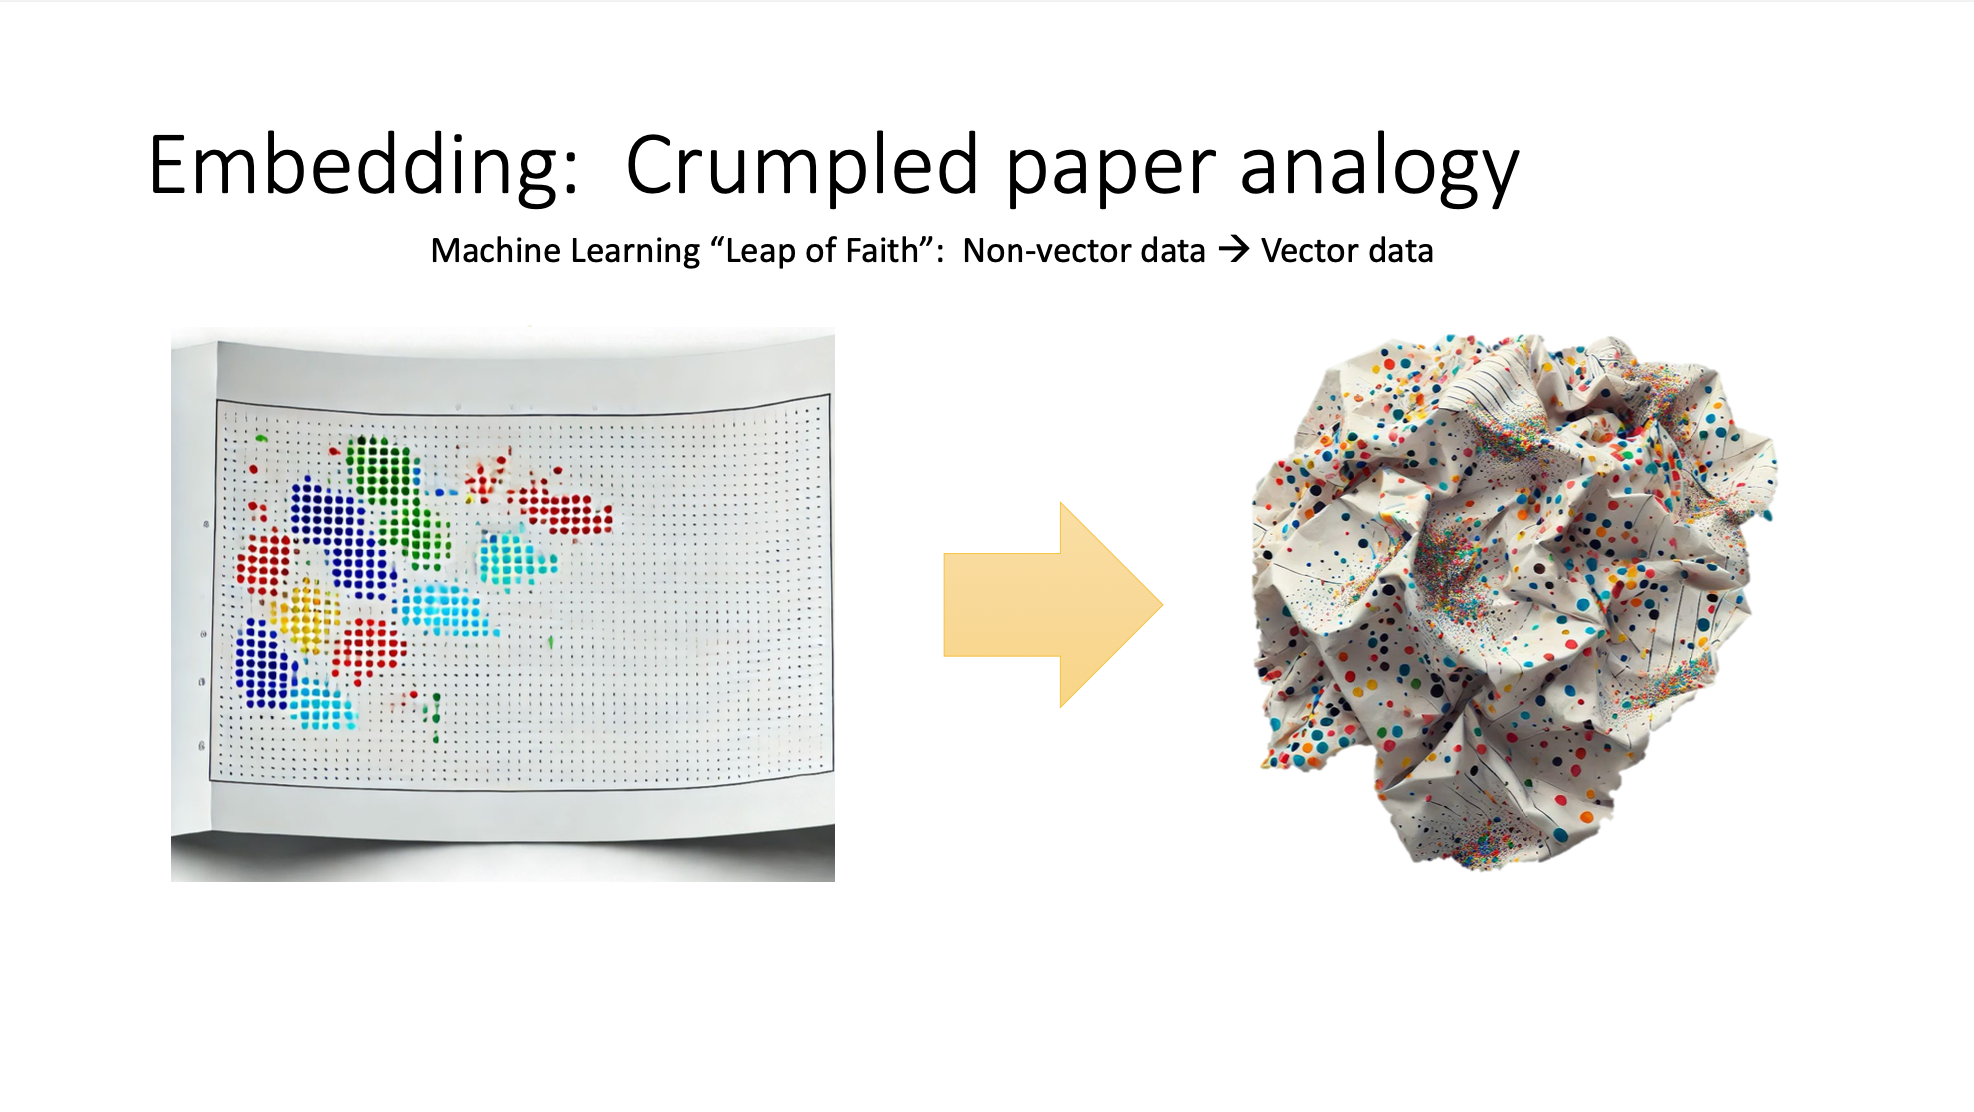
\includegraphics[width=\textwidth]{figures/B1_crumbled_paper.png}
    \label{fig:self_information_potential}
\end{figure}


And so it's like you've crumpled up a piece of paper
I cannot go anywhere in the data and say: 'Oh, I believe \textit{this}

\begin{equation}
    -\log{p_{similarity}(\mathbf{y}, \mathbf{y'}) \sim || \mathbf{y} - \mathbf{y'}||^2}
\end{equation}


is true.' In other words, then it's just a giant ball with Euclidean measures everywhere. This is not the case. This is only true locally. Okay? And you might—you might very correctly ask the question: 'Well, what the hell does that mean? Locally. What's local? How do I figure out what local is?' It turns out that's kind of the real problem you're solving—is what does local mean? 

\textbf{'Do I have enough data that I can believe in \textit{this}?}. \textit{This} is more of a belief that you can do this. Okay? It's sort of an ansatz or, you know, a postulate that you can do it.
So it's just a normalization trick in machine learning when they do that. But it's like: 'Do I have enough data to believe that I can make this true?' And if I don't, I'll just find out I just have this high-dimensional noise ball that I can never quite figure out what's going on with. 



\subsection{Data sufficiency is a \textit{local} question}


\begin{figure}[H]
    \centering
    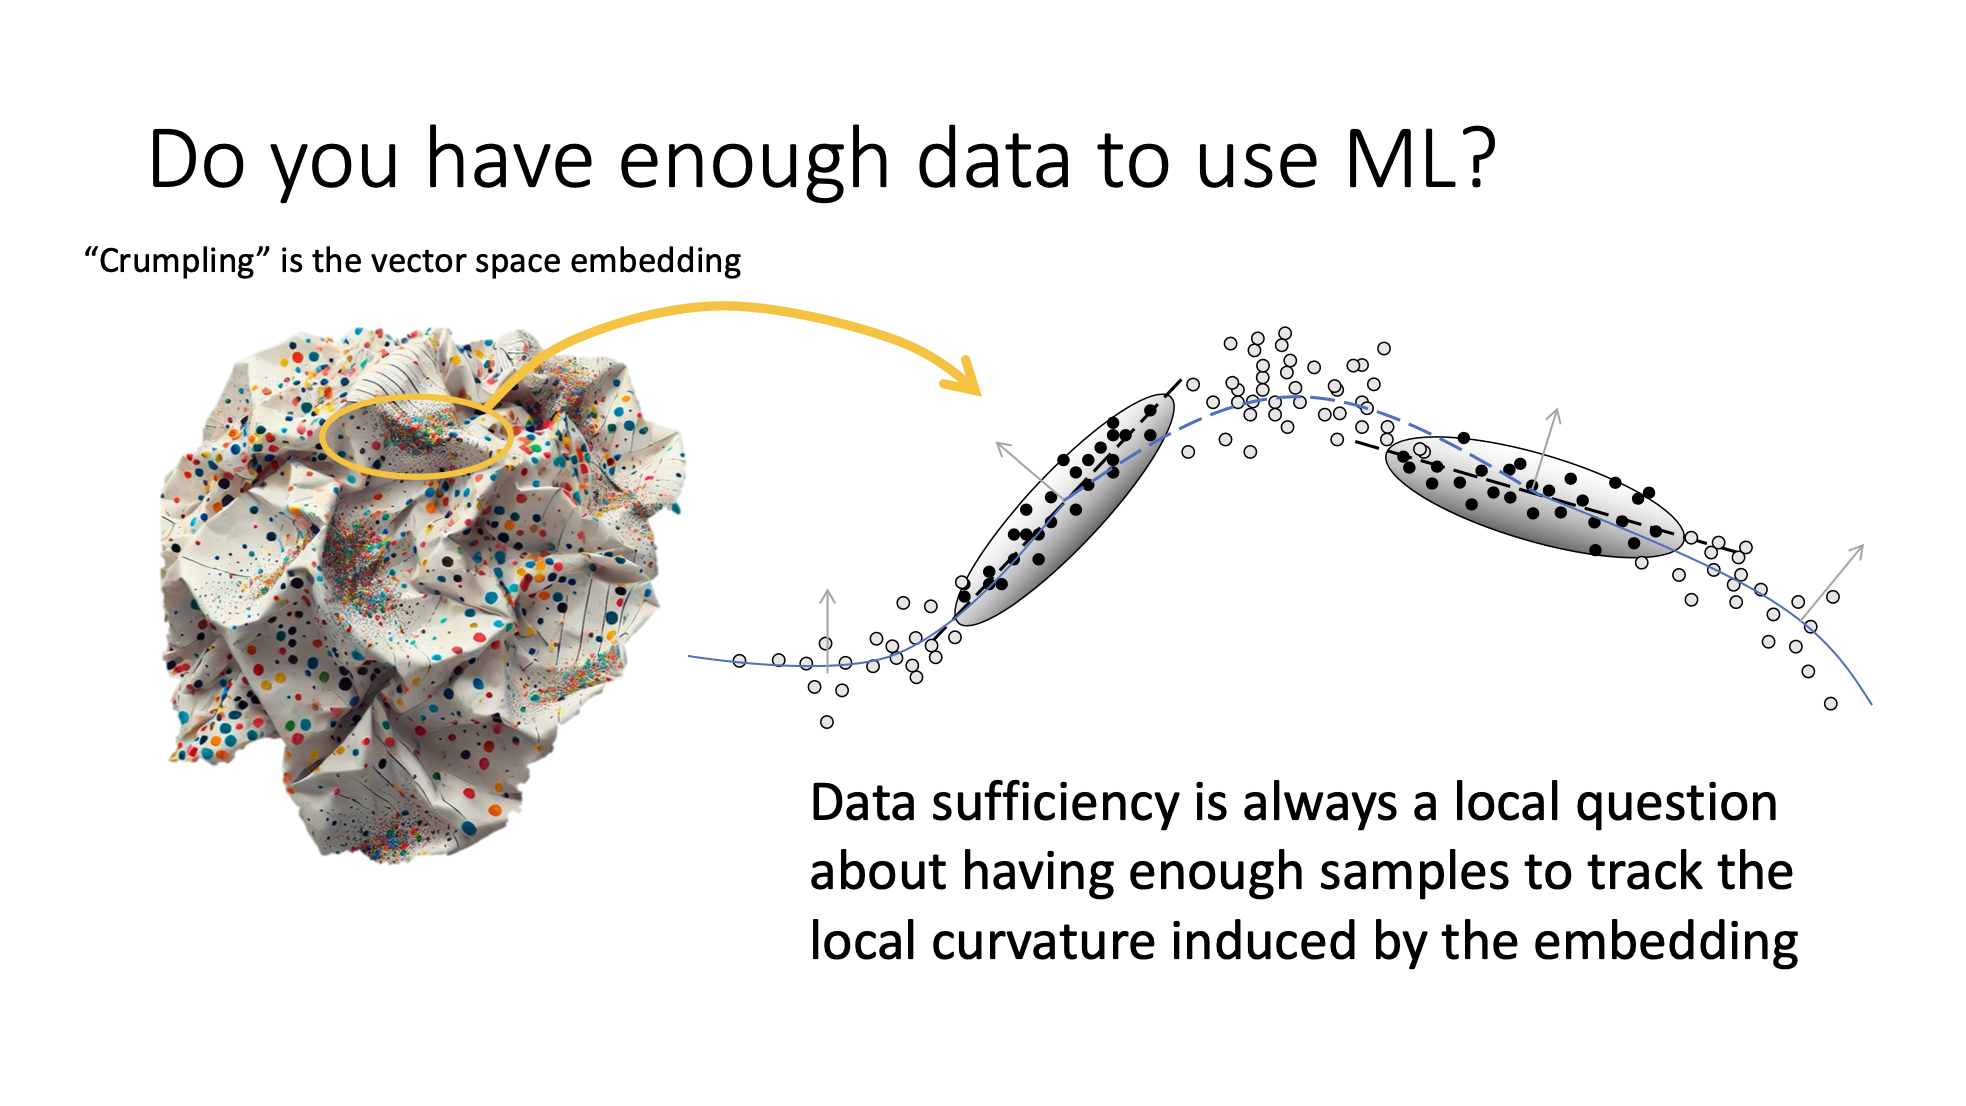
\includegraphics[width=\textwidth]{figures/B1_data_sufficiency_local_question.png}
    \label{fig:self_information_potential}
\end{figure}

\textbf{So what's the other thing they almost never talk about in machine learning? How do I figure out if I have enough data?} Did anyone ever explain that to you? How do you have enough data in machine learning? They have no idea. 

But I'm saying now you actually have a way to think about this, and it's related to the differential geometry that we are coming to, which is essentially the closeness or the farness compared to the curvature of the thing. 

So if the space is flat, then it probably doesn't take many points of data to sort of figure that out, right? So I have something here that's relatively flat sitting inside some space and maybe this thing here is lower dimensional than the space it's sitting in. Oops. Okay? But it's flat. If I believe it's flat, that's easy, right? Just a few points. But then this rule here applies everywhere in that space. You can use this all over this entire space. There's no problem. 

Now the problem starts... now we've got a different sort of space. So we have something that's more like a manifold and it may be inside of RD, but then we have a question like: 'Okay, well in some sense that we'll talk about, the dimension of this might be little d, like this up here,' but we have, you know, curvature, right? And so how many points do I need to learn this object versus this object? 

More. \textbf{This is a more complicated object. If you want to be more formal about it, it takes more parameters to identify this object than the number of parameters it takes to identify that object.}

So on this object, \textit{this [Euclidean distance]} is not true everywhere. But where is it true? Tangent spaces.

And that turns out to be what the essence of differential geometry is. It's very complicated objects embedded in a space, but the little pieces of the objects are like the Euclidean space you know and love. It turns out \textbf{manifolds are the most general place that you can still do calculus}. Those are the most general places that calculus is still functional in the form that you think of it from an undergraduate standpoint. 


Well, I've worked 20 years in machine learning, and the first question everyone always asks is, you know, "I have X amount of data, is it enough?". I've no idea, right? How could I possibly know the answer? \textbf{Because it's not the amount of data you have, it's where the data is}

So that's why you can't answer the question 'Is it enough data?' I have to say 'Given your embedding and understanding the amount of curvature in it, is the data placed correctly to find the structure that's hiding inside the embedding space?' All right. It just comes with the territory when \textbf{you say 'I turned my probability problem into a geometry problem' that, you know, nothing's quite for free. There's going to be some trouble that lives inside the other space, and curvature is kind of that trouble.}


\medskip \noindent 

So we've crumpled our paper — \textbf{and remember, in your data, you just have the points here, you don't have the paper. If you had the paper, your job would be easy} — just unfold the paper. 

But the paper doesn't exist. \textbf{You have to infer the paper from the points}. But notice the trouble here is when the paper got crumpled, there's lots of points that became very close to each other, but they're on different pieces of the paper. I have to be able to figure out the difference, by following the underlying structure. The paper is the manifold. Okay? 

And all I have is a point cloud. I have no manifold. \textbf{The manifold is a model concept. The data is what you have}. So, as I've already suggested here, we have a—a tool that we'll try to think about using—tangent spaces. And because on those tangent spaces, that's where the geometry actually works—on the tangent space. And so we have to be able to have the points to follow this around and then be able to say: 'Well, \textbf{how do I learn these tangent spaces?}

So that's the—the primary connection between differential geometry and machine learning. They both are—they—the machine learning induces a geometry from its probabilistic kind of problem, it induces this geometry, but then that geometry um has to be learned from just a point cloud. It's just a bunch of points in a space, there's no topology to it, there's nothing, it's just points. 


\begin{verbatim}
QUESTION: "how lower dimensional are tangent spaces?' 
'Is there a rule of thumb?' 
\end{verbatim}

No, I don't—but think of it this way. Think of the generative process that makes the data. And then ask how many parameters do you believe in are needed to be specified to make that data.  That is actually the dimensionality of the manifold the image sits on, in a sense.
So when you look at this you go where is the real world? Where is the stuff I'm trying to understand versus where are my models of the stuff? Well, think of it like I have a data space here. And what happens is that sensors create giant data spaces. And you might say well that's inconvenient. We wish sensors didn't create giant data spaces for us. But that's not true. The sensor creates this giant data space $R_D$. Like think of a camera. So I have a camera, you know, that's like 1920 by 1080 pixels, you know like HD, three color depths... it's like 6 million you know numbers to represent that. You're like wow that is... that's a 6 million dimensional space if you want to think of it that way. 

But remember very, very, very, very little of that space is actually used. Right? The space of natural images is like a wispy tiny thing hidden inside of that space that occupies very, very little of the actual space of all the dimensions that the sensor—the HD sensor—could actually see. And that's an important fact because you learn more from a sensor that could have seen anything but only saw this. That means that was like a lot of information content. Those choices—of what the sensor actually saw versus what it could have seen—is an incredible amount of information. 

So, the downside of it is you're... you're stuck though in this data space that's huge. Think of it like in statistical mechanics, like a phase space or something for dynamics. It can be quite huge, right? Six to the $n$ number of particles. So it's this massive space over there. 

But just like in physics and mechanics, you learn that there's only certain restrictions on that of the generative process, whether it's conservation of energy and how momentum works and symmetries like angular momentum. They all reduce the dimensionality and you can actually solve the problem because there's a model space that's lower dimensional so that you are not crushed by the curse of dimensionality. 

So have you all heard of the curse of dimensionality? Well, the important thing is to understand where does the curse live. The curse of dimensionality is never in your data. If your data has a curse of dimensionality, you're screwed. There's nothing you can do. It's over. Give up. There's nothing to fix it. Okay? Curses of dimensionality happen in your model. Your model has lots of degrees of freedom you have to prune and control and manage. And so the curse of dimensionality in your model space though is about regularization, right? You've heard regularization, or having a Bayesian prior, you know, or something. Like the log of the... of the Bayesian prior is sort of like the regularization in your neural network or your... your machine learning problem. 

And so over here in the model space you say well there's some sort of restriction that's going on here, and in large measure that's that dimensionality reduction we're talking about. How do we find that tangent space? How do we get down onto that manifold? How do we find the subspaces where that data really is living? Because those subspaces represent the fact that just in an example I was explaining to you about like the image of something, there's not that many parameters needed in the generation of the data, right? The sensor—the... the camera sensor—may have 6 million dimensions but I don't need 6 million dimensions—6 million parameters—to create the image. I may only need 50 parameters or 100 parameters. And that's the lower dimensional space that we're looking for here. 
\medskip \newline


\subsection{Locality and data attribution: Neural networks versus Kernel Methods}

\begin{figure}[H]
    \centering
    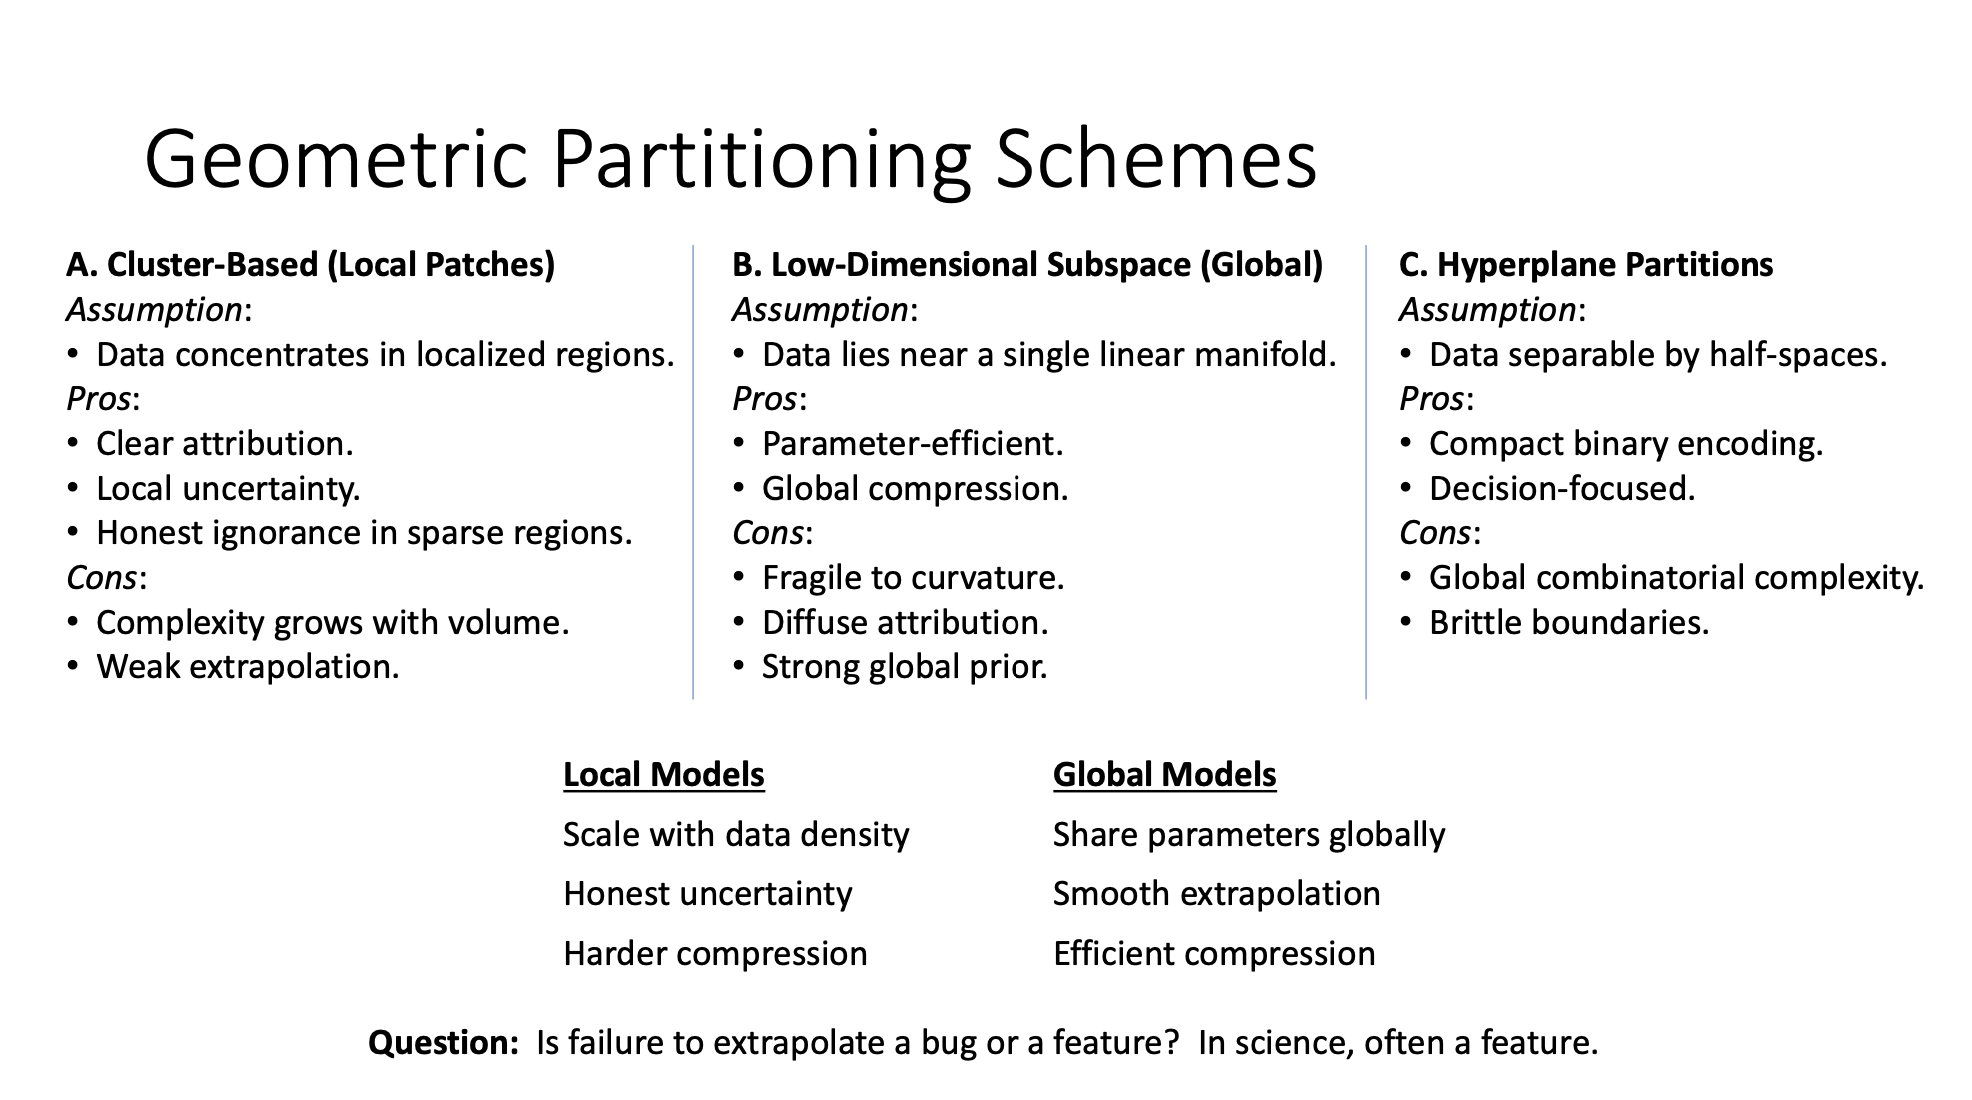
\includegraphics[width=\textwidth]{figures/B1_classical_ML_geom_schemes.png}
\end{figure}


\textbf{A neural network is a global fitting scheme, not a local fitting scheme.} So the neural network says: 'No, we're going to solve a problem this way.' It's going to chop the space up into half spaces essentially and talk about being on either side of those and it's almost like a zip code. To specify your position, you'll say you are on, you know, this side of that and that side of this and you'll sort of specify yourself essentially on the different sides of all these hyperplanes.

But notice what that means. And this is why neural networks are very bad for experimental science. Can you tell me where I should get more data?  Like I go and I do my project and I find out unfortunately for whatever reason my analysis doesn't really come through with the data I have, but now I would like to do some experimental design. I would like to get more data. And well the question is: 'Well, where would it matter to get more data? Where in this space do you need more data?' 

Well, if you're over here in this picture, where do I need more data? It's pretty clear. I'm tracking this curvature, I may not have enough data there and my local system here, like I didn't have enough points and I say 'Ah, I can't resolve this. It's just a ball. And this is just a noise ball here.  I did okay here, not good there.' So from an experimental design standpoint, I know where to go. 

Now I'm over here with my neural network. How does it tell me where to add the points? I don't know. Because it's every one of these pieces of the model. \textbf{It's a global cut across the entire data space.} So it's very hard for me to do um assignment of data, to say \textit{what} about my data created \textit{what} about my model.

I would claim you guys should be uncomfortable, somewhat unhappy with that approach and cautious. And the caution is that if I can't do data attribution and I can't do data sufficiency, well, you know what the next thing that I'm facing is? If I can't do those things, I can't do interpretation. 

In things like, you know, physics and chemistry and biology and the things we do, we're not looking for inscrutable black box, we want interpretability even if you have pretty good performance in the algorithm. So neural networks are very unfriendly to interpretability because of these problems with data attribution and data sufficiency. 

It's a geometric choice of how a neural network is constructed that creates this type of problem.


\begin{verbatim}
QUESTION: "'Could you maybe explain why the neural network is like slicing the space? 
Because I mean if we have access to the slices then we could like define the density,
and then we would know when we need data, right?
 Like the amount of data we have per space and if the density is low.'
\end{verbatim}



It's this vector W points in a place. The position of this plane is set by this bias piece right here. So think of it as like—let's pick... I don't have colored chalk, so I apologize for that, I'll have to work with white. I'll—let me make this double arrow thing like that. This double arrow is really saying what—where is it through the transformation of the weights, right? So I'm saying this is kind of like this arrow and then this is sort of setting well along this line where do I cut it to put the plane where the variation of the plane—now it's not—I take your point, it's not strictly like oh there's this plane sitting there. 

It's more like a plane that's blurred by the scale of the parameters of W. So it could become very blurred if the values here um become very large or it becomes very sharp. This allows you to do that. But what I'm pointing out is you—I mean you've seen this, this is the typical neural unit in your neural network, it's written this way, right? for a layer. And so this is the input layer, that's the output layer, so that's the input, that's the output. 

And so now we say: 'Here I am on the one layer and then I come out the other layer,' but it's kind of this object that gives the game away—the dot. Sigma dot. This is coordinateized. So you go into the coordinates of that thing and you pick off the first coordinate and use it. And then you pick off the second one and use it. 

So it's kind of like I line it up with something and then I cut, and I say all the data that's—figures out how to set the W and the B is the data on either side of where this arrow decided to point and where I would put the B. And so all the data on either side in principle, probably mostly near the boundary here, right here, that decides what happens here. So that cutting across the space is what creates the problem. 

\textbf{In other words, it's not like oh there's just a certain compact set that is controlling what happens to this piece of a model. The volumes involved here are essentially infinite.}
\medskip \newline
If there were a machine learning professor sitting in here, they would say: 'Oh, you're just trying to resurrect kernel methods over here.'  \textbf{A kernel is in general a compact object that localizes what data is involved in the model. So the kernel approach is sort of like the other road to travel.}
There's the neural network one, and then there's sort of the kernel-based approaches. And so I'm saying that the mathematics of understanding spaces is more aligned with kernels and those techniques than they are to neural networks. Even though machine learning and everything is mixed together and you can have kernels that live in neural networks in weird ways.
\medskip \newline


\subsection{We need to learn how to do \textit{local} PCA}


But the difference is that PCA just does it on everything. It's kind of dumb. It just takes the entire data set and says fine, we'll just do this spectral... the singular value decomposition on it. We'll find the singular values that are bigger, we'll keep those, we'll throw away the smaller ones, and that creates a projection matrix and then creates a subspace. And the projection matrix takes the data and puts it down on something like this tangent space. 

The problem is that if you did this for the entire data set, I mean what's going to happen? I mean it's kind of the wrong answer for all the data. It'll project it down but it'll destroy a lot of the intricate structure of your data. So the trick is: how do you do PCA in a slightly more intelligent way with a subset of the data? Okay? 

But it's not, but fundamentally it's no different than what you did with PCA when you just did it to all the data and just kind of projected everything down. Now granted, if I had this example over here, PCA is fine. If I do PCA on that object globally, it's no big deal. It'll find exactly what you need. It's a linear object, no problem. But if I do PCA on an object that has curvature in it, I could have a serious problem because the projection isn't really capturing the geometry of the object. And from a machine learning standpoint, it's not preserving that Euclidean distance effect that we were counting on to be able to do things. Okay. 



\section{Lecture 6: Differential geometry in ML, part II}

\subsection{\textit{Remark}: ML was developed for tasks that are essentially different from those in the physical sciences}
So think of it. A lot of those (ML) problems are things you can kind of just check because somehow your brain is very good at computer vision natural language processing. Right? So you can show up and, and saY: yeah, that's a good algorithm or a bad algorithm. But now, shift the context to science, engineering,, where if you knew the answer you wouldn't be doing the research. Right? And you're trying to use these kinds of algorithms and you're trying to also get some interpretation of the results of these, of the algorithm. And the, it's quite a big difference.

In a lot of science and engineering problems the embedding space means something. It could be a phase space, in a mechanics problem, it could be a, a more, slightly more abstract space in a genomics light problem, biology, it could be an engineering problem where it's a configuration space of possible, um, states of a mechanical system. And these, these things are taking place even in real spatial dimensions with other metadata layered on top of it. 

So that's why in one of the very first lectures over the, the Zoom ones, the first four I gave at the beginning, in one of those lectures I talked about how machine learning progressed from initially, um, having embedding spaces that were separately developed and then algorithms applied on top of them. That was the classical sort of machine learning world. But then deep learning was really the, the co-optimization of both embedding with the geometric algorithm on the vector space. Okay? And so now that's basically saying that you're saying I'm giving my algorithm the ability to change the geometry at will to support the problem it's doing. Now that is a huge difference. Okay? It means it's completely operationalized. It's, it's purely about optimizing a cost function now. So, let me tell you, if you want deep learning to be your problem, you better have really figured out your cost function because that's the only thing that connects your problem to what you're doing at that point. 

But if you're doing a physics problem and you say, well there's some background to the problem I want to do, let me ask you: do you want to preserve it in the geometry of your problem or do you want to try to make sure it's hiding somewhere in the cost function of your problem? Okay? That's the key difference. So, if you're in science and engineering, you want to respect embedding spaces more than the computer scientist does who wants to build a computer vision system or a natural language processing system. 

\subsection{\textit{Remark}: Noise is a \textit{modelling} choice}
But I think I emphasized this before too is like remember there's no noise in the world. The world doesn't have noise, the world doesn't have your model in it either. These are conceptual tools for you organizing your data. Noise is a modeling concept, not a thing in the world. Okay? Because sometimes noise changes depending on what you're doing. You make a different choice for what your problem is and the noise becomes different too. So don't ever get confused that there's like oh there's signal in the world and there's noise in the world and these are things the world picks. They're things you pick with your brain based on the problem you do. 

So when I say there's noise out in the codimensions perpendicular to this manifold, all I'm saying is I model it in some probabilistic way that doesn't cause me a lot of trouble. I say oh there's a Gaussian model that is that noise and I call the Gaussian model my noise in the problem, okay? So the next thing we want to know is how do we measure things. Remember this was the point of the geometrization of the data was that we said we don't want to do probability. Probability's hard. Probability calculus is difficult and, and expensive computationally. So we said hey I've got a great idea for machine learning which is instead I'll use numerical linear algebra because numerical linear algebra is one of the fastest things that we could run on a computer. 

So how do we turn probability problems into linear algebra problems? If you can do it, it's incredibly smart because the payoff computationally is huge. All right? This is really important. So that is what machine learning is. It's replacing probability with numerical linear algebra but when you do that, it's really saying instead of computing probability, I'm going to compute a geometry and I'm going to use distances in the space of the geometry as a substitute for what I meant about the probabilities. 


\subsection{The metric tensor}

\begin{figure}[H]
    \centering
    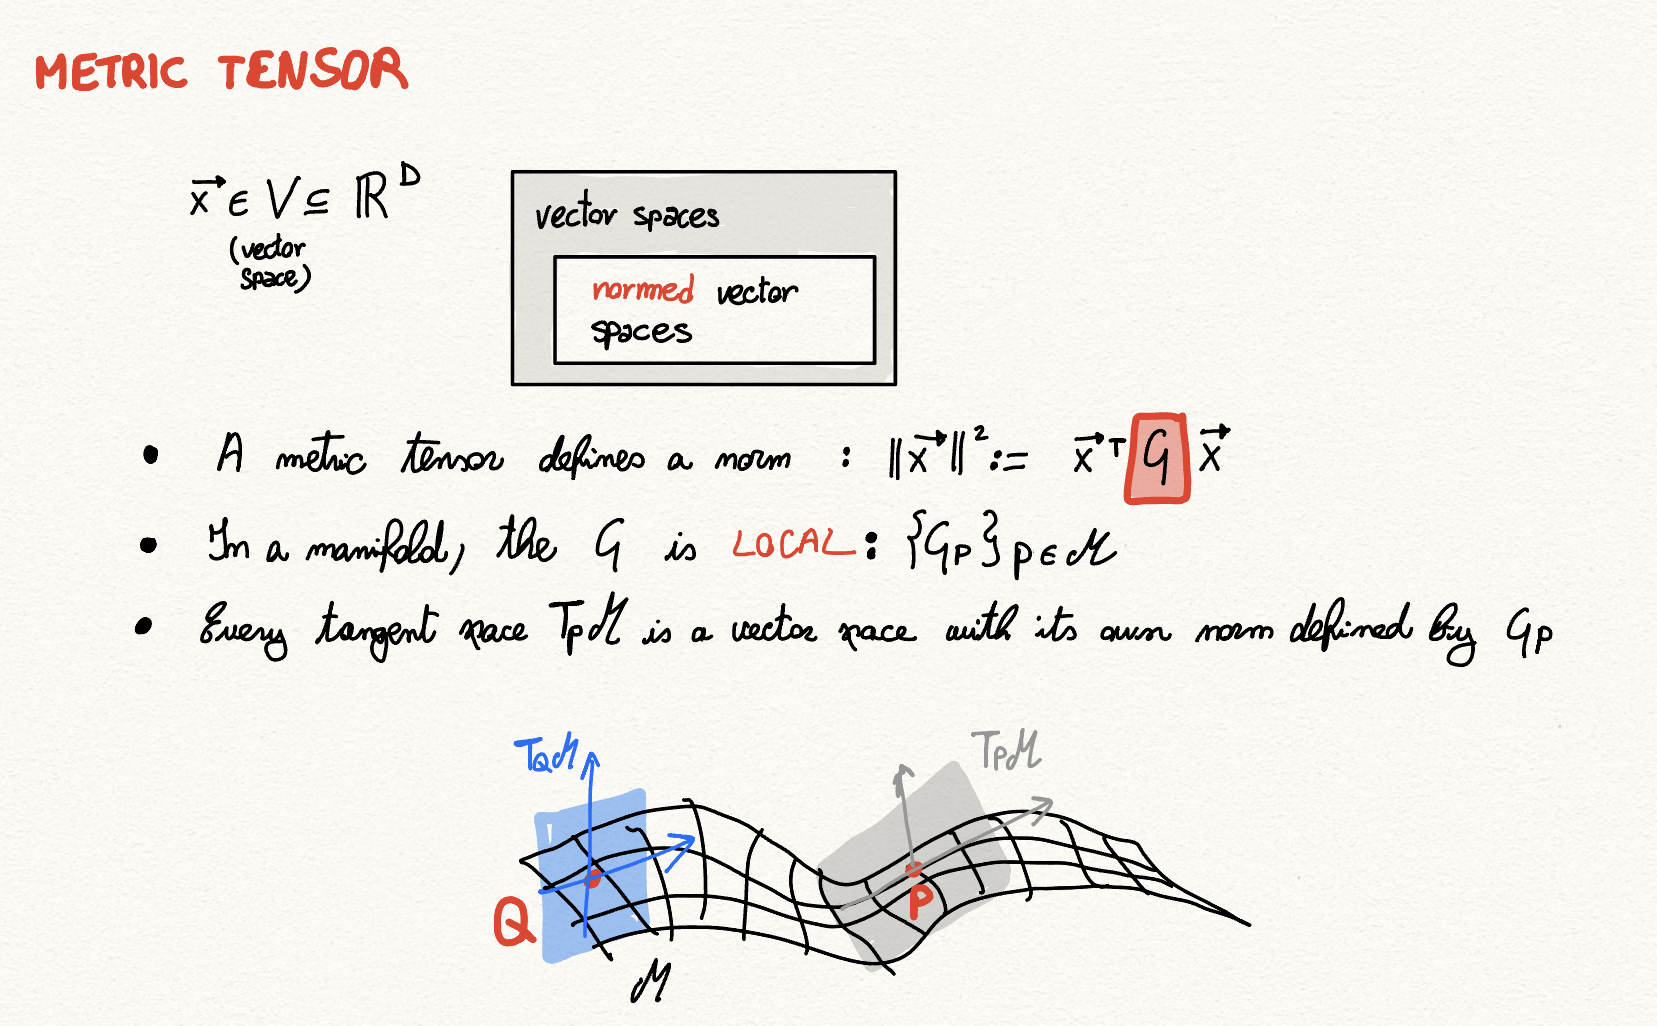
\includegraphics[width=\textwidth]{figures/B6_metric_tensor.png}
\end{figure}


With the tools just of what a vector space is, I can't tell you the length of the vector. That requires another concept, okay? A normed vector space is more information mathematically than just a regular vector space. This metric tensor is a fancy way of helping specify that. 

What's interesting about what differential geometry does is this is position dependent. So that object, how that inner product takes place around the space, depends on which tangent space you're on. So if I go here and I say I'm doing this vector operation, it means that I have to say that this vector space actually is the tangent space of the manifold at some point P. Okay? And so I'm identifying it as I could have this crazy looking object, this manifold, but at every point I say there's a little piece of Euclidean space sort of glued there. 

And the Euclidean space is your friend, right? It's not tricky. It's a friendly vector space that just sits at the point P and you can exploit the properties of it. And one of the properties is on that particular space at P, not P here but identify that it is something that changes as I move around in the space, that I can compute this norm on that vector space that is that tangent space. Okay, this is the central idea of how I measure things in this world of differential geometry. 

\paragraph{Parallel Transport}
Got it? Helpful? Now, now let's say I had those vectors here and then I go over here to Q. Now I'm at TqM and you say 'well then I say oh well I have a vector here and I would like to know the inner product between a vector, uh, W that's an element of that space as compared to a vector V that's an element of this space.' And you'd say well how the hell do you do that? Right? Because they are... that's a different vector space than this one. And so as a part of what goes on in a lot of differential geometry, a very important aspect of it is what's called parallel transport. So it's the notion of how do I take vectors that sit on this complicated object and how do I move them around so that I could compare them? And it's not trivial. Okay that's not trivial at all. And so how you do the transport of this along the manifold is sort of saying 'well how do I make this sit in a... they have to sort of be in the same vector space somehow.' So I either have to figure out how do I parallel transport this vector V over to W and then use that rule, using the G over here? There's going to be a Gq here, there's going to be a Gp over here. 
\paragraph{The metric tensor variation describes \textit{curvature}}
And the variation of this metric tensor as you move around the space, that ends up derivatives of it that define what curvature is. That's the curvature, it's representing the curvature of the object we're talking about. But it also represents how do we figure out geodesics. om P to Q and the minimum distance possible. 
\paragraph{Defining vector fields on manifolds: tangent bundles}
Yeah and so now I can define vector fields on manifolds. Okay? But it says 'well they are vectors only on each of the tangent spaces.' You know there's a complicated concept called a tangent bundle that I'm not going to get into it right here but the tangent bundle and doing sections of it shows you how you put vector fields on objects like this. So it really is, the manifold is kind of the last place where you get to use all the stuff you learned in vector calculus. All that, all the differentiation and integration and all those kinds of things, they still work on these objects. They're kind of the last place they do. 


\paragraph{Tensors are the \textit{real} things}
Remember we wanted to figure out how to, um, make observations about reality. Okay, my reality in scare quotes I just mean things that are not contaminated by choices we make. 

What we can do is always ask that when we put different coordinates onto our problem, the transformation between the, the coordinates leaves invariant the things we're claiming about the, the manifold world up here. And so by being able to say there are objects that the, the, you know, the chart transi- chart transition maps leave invariant when you look at them on the manifold, tells us these are like real objects. These are the things we should be talking about in physics or whatever problem we're doing. 

But in physics and engineering, the objects that can live up here and obey this notion of being able to withstand the chart transition maps and being invariant to them, remember I told you what they are: those are the \textbf{tensors. That's what tensors are. This is why tensors show up so much and why they're so important. They're the objects that survive the chart transition maps here and are candidates to actually be up there on the, the manifold, you know, the, the plane of reality so to speak}. 

\subsection{Our intended pipeline to learn the manifold}
\begin{figure}[H]
    \centering
    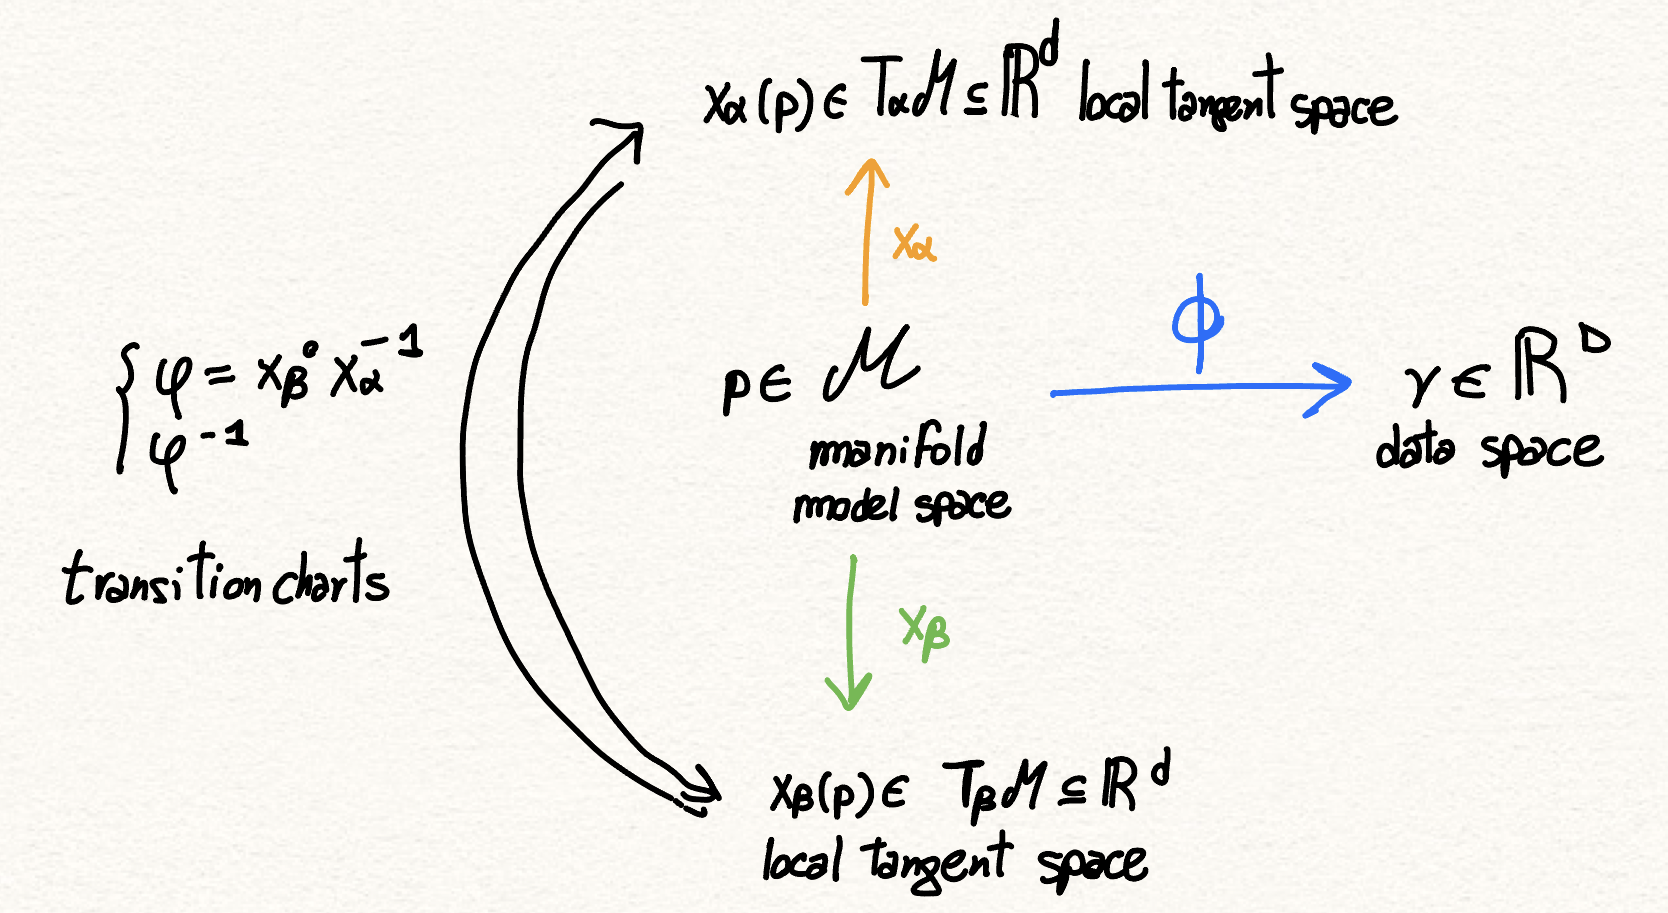
\includegraphics[width=\textwidth]{figures/B6_goal.png}
\end{figure}

\begin{enumerate}
    \item Location: where is the tangent space anchored?
    \item Dimensionality: how can we reliably infer the dimension of tangent spaces from finite-sample data?
    \item Scale: How large is the curvature of the manifold at that point? Therefore, how far from $P$ can we approximate $\mathcal{M}$ with that tangent space $T_p \mathcal{M}$?
\end{enumerate}


So now we have to say how do we do PCA to find this tangent space and the dimensionality of it, but we have a finite number of samples, okay? We only have so many samples to use, we don't have the entire data set. So we have to actually confront the fact that we're going to have finite sampling noise when you try to do this.

And so I can ask about the scale here. So the scale is saying well maybe it's very flat where I am and so that tangent space actually is a really good approximation over a large area of that manifold. Okay so that local model answers the question over a significant area. Or, oppositely, it's in a very curved area, right? And the curvature says well the scale of where I can use that tangent space is actually quite small, okay? So I have to shrink it in quite a bit and reduce the scale to be able to to use that tangent space. But that's a function of the curvature of the manifold. 


\paragraph{Spectral gap in the data covariance matrix}
So these three issues they can be... this first one can be addressed just by saying okay just pick enough points to cover the manifold. These two relate more towards computing relevant statistics about the point cloud locally, like the sample covariance matrix, okay? We'll take a look at that. I just wanted to remind you something I know you already know. You probably have done a singular value decomposition many times. And I'm just reminding you about it um so that we're on the same page or maybe there are my notation lines up with how your notation was in your courses. 

And now we're going to look at the eigenvalue spectrum. So initially if I don't have enough points to say anything I think well I don't know I'm in N minus one dimensions or I'm in big D dimensions if I have more points than dimension. And that just means it's a noise ball, it's a full dimension noise ball. I don't see anything, I don't detect anything, I don't see a tangent space, I'm just temporarily stuck. But as I grow this ball and I get into more and more data, I should start to see a difference between the directions that are bounded in the codimension. Right if it's a manifold there'll be directions that are bounding me and then there'll be other directions I can grow into because they are along the manifold. 

And so the growing of the ball will will detect a manifold by looking at the eigenvalue spectrum and what we're hoping for to see is an opening of a spectral gap. The spectral gap says there are some of these eigenvectors that are spreading out in directions of and those are the basis of the tangent space. That's all. Hopefully you see that this is nothing crazy or different, other than we just did it locally. And \textbf{the trick is to figure out well how do you pull it off statistically with just a limited amount of data}. That's the essence of what our problem turns into. We don't get to use all the data, we just use a little bit of the data, how do we solve the problem? 


\subsection{Q and A}


\paragraph{Q1} Assuming you succeed in learning a set of local tangent planes, then how do you stick them all together?

Let me do something naive that can still be very valuable: think of it as a lookup table. So if you say, well, I give a point and then I can say, "ah, in my lookup table now, I can say that point lives in this tangent space and it has this geometric structure." I don't necessarily have to stitch it all together. I mean, remember, machine learning has set a low bar. They don't... they don't do anything with the geometry whatsoever. And if I can at least tell you, give me some new point or say, "at this point in my data space is there a manifold? One?" and like data support, "is there anything there first?" And the other thing is, "okay, if there is something there, tell me about the degrees of freedom and how they sit within the overall space." That's actually pretty good as a starting point. But we'll come to this other question in just a little bit too. I agree, it is a hard question.

\paragraph{Q1} In the landscape of state-of-the-art machine learning methods, is there already some well-defined, well-structured method that uses this way of thinking and was effectively been applied to a problem in the physical sciences?

So, most of the work that goes on now is not geometric. If you go back though, twenty years, as more of the classical machine learning, that's where you did find the techniques like \textit{local linear embedding (LLE), Isomap, LTSA (Local Tangent Space Alignment)}.  So I sort of answered your question. Sort of. So it isn't... it's a little bit of an open topic, and it also, as it was developing, it all got steamrolled over by deep learning, because deep learning happened soon after those early innovations. So but I think it's time to kind of come back to it for science and engineering problems. 